\documentclass[a4paper,oneside]{article}
%Compilé avec MacTex
\usepackage[french]{babel}
\usepackage[utf8]{inputenc}
\usepackage[T1]{fontenc}
\usepackage{hyperref} % références dans pdf
\usepackage[tt]{titlepic}
\usepackage{graphicx} % pour images
\usepackage{rotating} % pour rotatebox
\usepackage{lmodern}
\usepackage{amsmath}
\usepackage{amssymb}
\usepackage{mathrsfs}
\usepackage{sistyle}
\usepackage{chngpage}
\usepackage{caption}
\usepackage{epstopdf}
\usepackage{gnuplottex}% pour faire du gnuplot directement dans le latex
\usepackage[nottoc, notlof, notlot]{tocbibind} % pour que bibliographie soit comprise comme un chapitre ou section
\usepackage{appendix} % pour les annexes
\pagestyle{headings} % pour en têtes
\usepackage{mathenv}
  %\usepackage{SIunitx}
%\usepackage{siunitx}%pour les unités SI
\DeclareTextSymbol{\degre}{OT1}{23} %pour le symbole degré
\makeatletter % pour /bigcenter qui permet de s'affranchir des marges pour les images
\newskip\@bigflushglue \@bigflushglue = -100pt plus 1fil

\def\bigcenter{\trivlist \bigcentering\item\relax}
\def\bigcentering{\let\\\@centercr\rightskip\@bigflushglue%
\leftskip\@bigflushglue
\parindent\z@\parfillskip\z@skip}
\def\endbigcenter{\endtrivlist}
\makeatother


\begin{document}

%************************************************************************
%									TITRE
%************************************************************************


\begin{titlepage} % Suppresses headers and footers on the title page

	\centering % Centre everything on the title page

	\scshape % Use small caps for all text on the title page

	\vspace*{\baselineskip} % White space at the top of the page


	\rule{\textwidth}{1.6pt}\vspace*{-\baselineskip}\vspace*{2pt}
	 % Thick horizontal rule
	\rule{\textwidth}{0.4pt} % Thin horizontal rule

	\vspace{0.75\baselineskip} % Whitespace above the title

	{\LARGE Bureau d'\'Etudes :\\
	\vspace{0.75\baselineskip}
	Conception d'un Réacteur Chimique\\
	} % Title

	\vspace{1\baselineskip} % Whitespace below the title
	\rule{\textwidth}{0.4pt}\vspace*{-\baselineskip}\vspace*{3.2pt}
	 % Thin horizontal rule
	\rule{\textwidth}{1.6pt} % Thick horizontal rule
	\vspace{2\baselineskip} % Whitespace after the title block

	%------------------------------------------------
	%	Subtitle
	%------------------------------------------------

	% Subtitle or further description
	Méhodes Numériques : Volumes Finis

	\vspace*{3\baselineskip} % Whitespace under the subtitle

	%------------------------------------------------
	%	Editor(s)
	%------------------------------------------------


	\vspace{0.5\baselineskip} % Whitespace before the editors

	{\scshape\Large Quentin Bergé \\ Adrien Autellet\\} % Editor list

	\vspace{0.5\baselineskip} % Whitespace below the editor list

	\textit{ENSEEIHT} % Editor affiliation

	\vfill % Whitespace between editor names and publisher logo

	%------------------------------------------------
	%	Publisher
	%------------------------------------------------

	
\includegraphics[scale=0.3]{logoN7.png} % changer logo

	\vspace{0.3\baselineskip} % Whitespace under the publisher logo

Juin 2019 % Publication year
\end{titlepage}
\newpage

%Table des Matières
\tableofcontents
\newpage

\section{Introduction}

L'objectif de ce bureau d'études est d'étudier la cinétique chimique lors de l'injection de deux réactifs au sein 
d'un réacteur chimique. Cette cinétique étant fortement influencée par la température, on se propose d'étudier le phénomène 
d'advection-diffusion de cette dernière par la méthode des volumes finis.

\section{Description du Problème}

Selon la configuration schématisée dans la figure ci-dessous, les deux réqctifs sont injectés face-à-face.
Puisque la diffusivité thermique des réactifs est très grande, l'efficacité de l'échangeur est dictée par la cinétique de la réaction qui est très influencée par la température. Cela revient donc à étudier le champ de température sur toute la taille du réacteur mais surtout dans la zone centrale. C'est pour cela que nous analyserons le phénomène d'advection-diffusion de la température par la méthode des volumes finis. 


\begin{figure}[h!]
\bigcenter
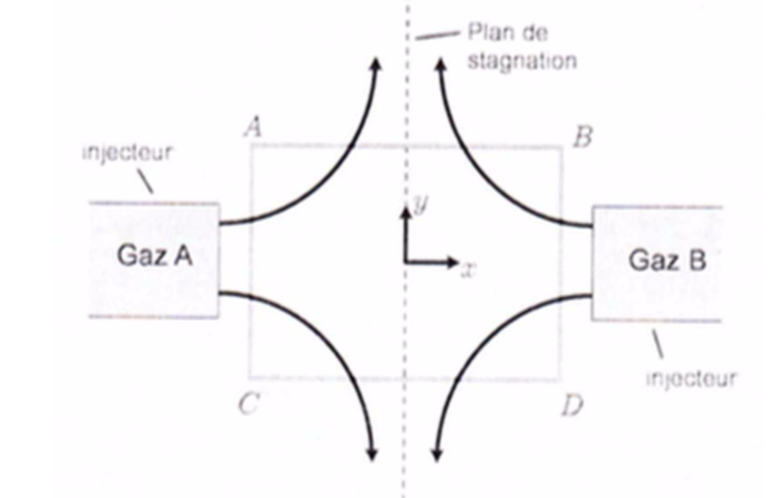
\includegraphics[scale=0.8]{Schema_reacteur.PNG}
\caption{Schéma du système d'injection dans le réacteur chimique}
\end{figure}

Selon le cahier des charges, nous devons respecter certaines scpécifications :
\begin{itemize}
	\item Maillage irregulier en x et y
	\item Schéma amont pour le terme advectif
	\item Schéma centré pour le terme diffusif
	\item Intégration temporelle par la méthode d'Euler explicite
	\item Conditions de Dirchlet avec température gaussienne sur les frontières AC et BD
	\item Conditions de Neumann avec Interpolation des flux diffusifs à partir des flux connus à l'intérieur du domaine\\
\end{itemize}

L'équation de transport des températures s'écrit alors :

\begin{equation}	\label{eqderivpart}
\frac{\partial T}{\partial t} + \nabla . (\overrightarrow{U}T) - \nabla . (\alpha \overrightarrow{\nabla}T) = 0 
\end{equation}

\section{Pré-Processeur}
\subsection{Lecture d'un Fichier d'Entrée}

Le fichier d'entrée est disposé dans le dossier RUN et donne accès à certaines variables que l'on peut changer comme des Données Numériques :
\begin{itemize}
	\item temps final
	\item nombre de points en x $N_x$
	\item nombre de points en y $N_y$
\end{itemize}

et comme Données Physiques :
\begin{itemize}
	\item la longueur du domaine \verb?L?
	\item la vitesse carcatéristique des gaz $A$
	\item les coefficients de diffusivité thermiques $\alpha_a$ et $\alpha_b$
\end{itemize}

Ce fichier d'entrée est lu à l'aide de la subroutine \verb?read_data?



\subsection{le Maillage}
Etant donné que nous travaillons avec un code 2D il nous faut mailler le réacteur selon le schéma suivant.
Et puisque la subroutine de transformation de VTS vers Paraview nous fait utiliser des tableaux de taille ($N_x$,$N_y$), nous avons choisit cette structure pour tous nos tableaux.

\begin{figure}[h!]
\bigcenter
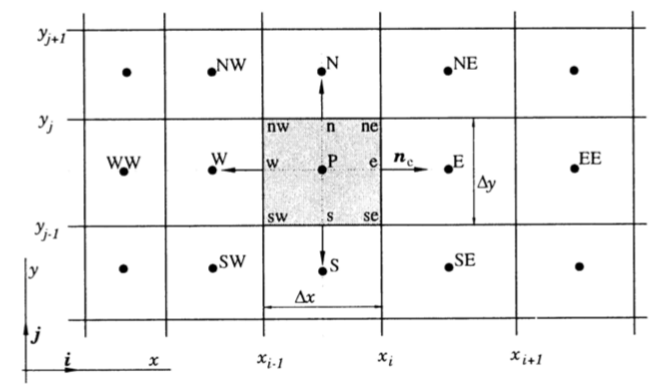
\includegraphics[scale=0.5]{Champ_Vitesse_Maillage/MaillageTheorique.PNG}
\caption{Exemple d'un maillage 2D SOURCE A METTRE Poly Alexei Stoukov}
\end{figure}

Pour ceci nous allons donc utiliser plusieurs tableaux, pour chaque maillage il y aura un tableau pour $x$ et un selon $y$ dépendant de ($i$,$j$) conformément au schéma ci-dessus.

Nous définissons alors 4 maillages différents :
\begin{itemize}
	\item pour les noeuds \verb?xnoeuds? , \verb?ynoeuds?
	\item pour les centres des volumes \verb?xcentre_vol?, \verb?ycentre_col?
	\item pour les faces horizontales \verb?xcentre_faces_horiz?,\verb?ycentre_faces_horiz?
	\item pour les faces verticales \verb?xcentre_faces_vertic?, \verb?ycentre_faces_vertic?
\end{itemize}

On effectue d'abord le maillage sur les noeuds et les centres des volumes, puis on peut composer les faces horizontales et verticales avec ceux-ci.
Tout ces tableaux sont de tailles différentes puisqu'il y a $N_x \times N_y$ noeuds mais ($N_x -1 )\times (N_y -1$) centres.
C'est pourquoi il faudra faire attention à la taille des tableaux quand on les allouera.
Ces tableaux sont en allocations dynamiques, on alloue uniquement la mémoire qui sera nécéssaire aux tableaux afin de ne pas trop en consommer en accord avec les données du fichier d'entrée. 


Etant donné qu'on lit sur le fichier d'entrée $N_x$,$N_y$, on va calculer les pas \verb?dx? et \verb?dy? 
\[
 d_{x,y} = \frac{L}{N_{x,y} -1}
\]

De cette façon on a pu obtenir un maillage régulier visualisé comme ceci avec ParaView.

\begin{figure}[h!]
\bigcenter
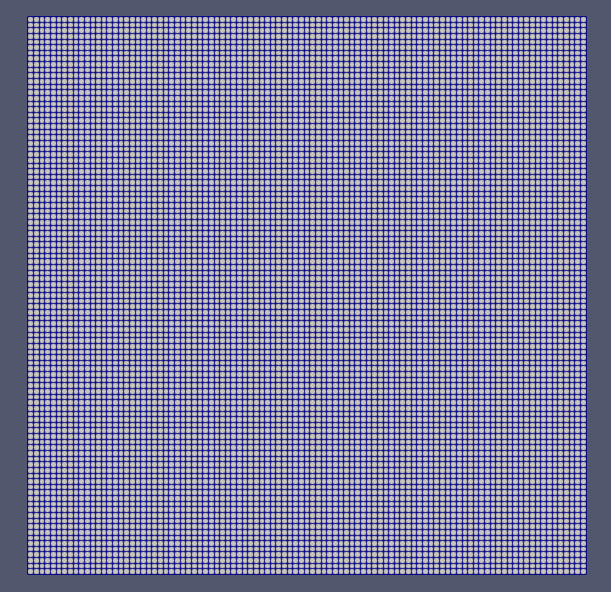
\includegraphics[scale=0.4]{Champ_Vitesse_Maillage/maillage100100.PNG}
\caption{Maillage (100,100) visualisé sur Paraview}
\end{figure}

Ce maillage est réalisé à l'aide de la subroutine \verb?maillage?

\subsection{Champ des Vitesses}

On a ensuite pu calculer le champ des vitesses aux centres des volumes selon \label{eqvitesses}

\begin{equation*}
\begin{cases}
 u = A \cos \left( \pi \left( {\frac{x}{L} - \frac{1}{2}} \right) \right)  \sin \left( \pi \left( \frac{y}{L} - \frac{1}{2}\right) \right) \\
 v = -A \sin \left( \pi \left( {\frac{x}{L} - \frac{1}{2}} \right) \right)  \cos \left( \pi \left( \frac{y}{L} - \frac{1}{2}\right) \right) \\
\end{cases}

\end{equation*}

 $A$ paramètre caractéristique de la vitesse maximale du gaz, ici choisi à 0,05 $m/s$.\\

Ce calcul du champ des vitesses est réalisé à l'aide de la subroutine \verb?champ_vitesse?

\subsection{Calcul du Pas de Temps}

Les calculs utilisant la formulation Volumes Finis nécessitent de calculer le pas de temps, étant donné que ce pas de temps $dt$ donne une condition de stablilité sur ce modèle. On le calcul de cette façon :

\[
	dt =  \left\{ \frac{\mid u_{min}\mid}{d_x \times CFL} +\frac{\mid v_{min}\mid}{d_y \times CFL} + \frac{\alpha}{r}\left(\frac{1}{d_x^2} + \frac{1}{d_y^2}\right) \right\}^{-1}
\]

\noindent $CFL$ est le nombre de courant, pris égal à 1\\
$r$ est le nombre de Fourier, pris égal à 0.5\\
$\alpha$ est le coefficient de diffusivité thermique qui est en réalité $\alpha_{moyen}$ que nous définissons comme $(\alpha_a + \alpha_b)/2$\\

En pratique on utilisera directement les fonctions intrinsèques présentes dans Fortran \verb?ABS? et \verb?MINVAL? qui nous donneront la valeur absolue minimale du tableaux u et v.
$CFL$,$r$,$\alpha_a$ et $\alpha_b$ sont modifiables dans le fichier d'entrée.

\subsection{Para View}

Para View est un logiciel libre de visualisation de données. 
Il nous permet à l'aide de la subroutine fournie \verb?VTSWriter? en fournissant certains arguments d'afficher nos résultats dans un format lisible par ce logiciel.

\section{Discrétisation}
Si on se restreint à un seul volume du maillage on peut représenter les flux comme ceci :

\begin{figure}[h!]
\bigcenter
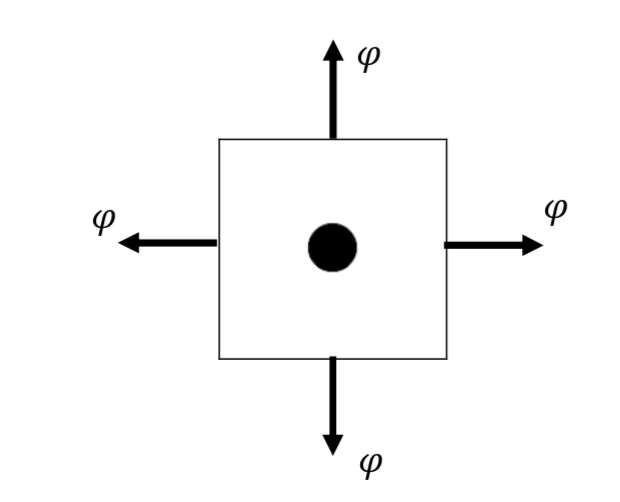
\includegraphics[scale=0.4]{flux.PNG}
\caption{Schématisation des flux sur un volume du maillage}
\end{figure}


Il s'agit donc d'un calcul qui s'effectue à chaque centre des faces et non au centre des volumes comme c'est couramment le cas pour les températures et les vitesses.


\subsection{Calcul des Flux}


Les flux advectifs et diffusifs dans le réacteur chimique se sont définis comme ceci :
\begin{equation*}
\begin{cases}
\phi_{adv} = \overrightarrow{u}\times \rho C_p T\\
\phi_{diff} = -\alpha \overrightarrow{\nabla} T\\
\end{cases}
\end{equation*}


En intégrant alors l'équation \ref{eqderivpart}, on obtient :

\[
\frac{d}{dt} (Volume_{i,j} T_{i,j})= \int \overrightarrow{U}T.\overrightarrow{n} dS + \int (\alpha\overrigtharrow{\nabla} T).\overrightarrow{n} dS
\]

Cette intégrale laisse apparaître alors une distinction selon les sens des normales donc le sens de parcours de notre maillage pour les flux advectifs mais aussi pour les flux diffusifs.
On va donc renommer les flux selon leur directions avec haut, bas, gauche et droite.

On obtient alors comme équation générale :
\begin{align*}
\frac{d}{dt} (Volume_{i,j} T_{i,j}) &= \phi_{adv,haut,i,j}dx + \phi_{adv,bas,i,j}dx + \phi_{adv,gauche,i,j}dy  \\
&+ \phi_{adv,droite,i,j}dy + \phi_{diff,haut,i,j}dx + \phi_{diff,bas,i,j}dx  \\
&+ \phi_{diff,gauche,i,j}dy + \phi_{diff,droite,i,j}dy
\end{align*}
\subsubsection{Flux Advectifs}

En notant que :

\begin{equation*}
\begin{cases}
	\phi_{adv,haut,i,j} = -\phi_{adv,bas,i,j+1}\\
	\phi_{adv,gauche,i,j}  = -\phi_{adv,droite,i,j+1}\\
\end{cases}
\end{equation*}

On va alors distinguer uniquement les deux flux advectifs 
$\phi_{adv,x}$ et $\phi_{adv,y}$.

On obtient alors pour $\phi_{adv,x}$ :

\begin{equation*}
\begin{cases}
	U_{i,j}T_{i,j} \ si \ \overrrightarrow{U_{i,j}}.\overrightarrow{n} \geq 0 \\
U_{i+1,j}T_{i+1,j} \ si \ \overrrightarrow{U_{i,j}}.\overrightarrow{n} \leq 0 \\
\end{cases}
\end{equation*}

De même pour $\phi_{adv,y}$ :
\begin{equation*}
\begin{cases}
	U_{i,j}T_{i,j} \ si \ \overrrightarrow{U_{i,j}}.\overrightarrow{n} \geq 0 \\
U_{i,j+1}T_{i,j+1} \ si \ \overrrightarrow{U_{i,j}}.\overrightarrow{n} \leq 0 \\\end{cases}
\end{equation*}
\subsubsection{Flux Diffusifs}

A l'instar des flux advectifs, on obtient des résultats identiques sur les flux diffusifs, seuls l'expression change :

\begin{equation*}
\left\{
 \begin{array}{c }
  phi_{diff,x,i,j}  \\
 phi_{diff,y,i,j}  \\
  \end{array}
\qquad
\equiv
\left\{
\begin{array}{c c c}
\alpha\frac{dT}{dx} = \alpha \frac{T_{i+1,j}-T_{i,j}	}{X_{i+1,j}-X_{i,j}}\\
\alpha\frac{dT}{dy} = \alpha \frac{T_{i,j+1}-T_{i,j}	}{Y_{i,j+1}-Y_{i,j}}\\
\end{array}
\end{equation*}

\subsection{Conditions Limites}


Les calculs décrits jusqu'à présent étaient définis sur tout le centre du réacteur chimique, maintenant nous allons nous attarder sur les extrémités en prenant en comptes les conditions limites pour le calcul des flux advectifs et diffusifs mais aussi pour les températures.

\subsubsection{Températures}

Les températures aux extrémités droites et gauches du réacteur notées respectivement \verb?TfaceAC? et \verb?TfaceBD? sont définies selon un profil gaussien :

\begin{equation*}
\begin{cases}
T_A(y)=(T_A - T_0)\e^{\frac{-y^2}{2\sigma_A^2}} +T_0\\
T_B(y)= (T_B - T_0)\e^{\frac{-y^2}{2\sigma_B^2}} +T_0\\
\end{cases}
\end{equation*}

$\sigma_A$ et $\sigma_B$ correspondent à $\frac{L}{20}$ et $T_A$,$T_B$ et $T_0$ sont modifiables dans le fichier d'entrée du programme.

Ces températures interviennent ensuite dans le calcul des flux aux extrémités de notre maillage.

\subsubsection{Flux}

Les deux flux ont en commun d'avoir les mêmes conditions limites pour les extrémités hautes et basses.
En réalité l'énoncé indique une interpolation des flux diffusifs à partir des flux connus à l'intérieur du domaine.

On va appliquer cette hypothèse pour les deux flux ainsi, 

\begin{equation*}
	\begin{cases}
		
	\phi_{adv,i,npty} = \phi_{adv,i,npty-1}\\
	\phi_{adv,i,1} = \phi_{adv,i,2}\\
	\phi_{diff,i,npty} = \phi_{diff,i,npty-1}\\
	\phi_{diff,i,1} = \phi_{diff,i,2}\\
	\end{cases}
\end{equation*}

\paragraph{Advection}
Pour les flux advectifs, nous définissons les flux aux points sur l'extrémité gauche comme étant le produit de la température du profil gaussien et de la vitesse au point :

\[
 \phi_{adv,1,j} =U_{1,j}T_{A,j}
\]


En ce qui concerne l'extrémité droite, nous considérons qu'il s'agit d'un flux sortant, c'est pourquoi nous calculons sa valeur à l'aide des vitesses et températures aux points précédents.
  
\[
 \phi_{adv,nptx,j} =U_{nptx-1,j}T_{B,j}
\]  


\paragraph{Diffusion}


Pour les flux diffusifs, les deux extrémités prennent en compte les profils de température $T_A$ et $T_B$.

\begin{equation*}
	\begin{cases}
		\phi_{diff,1,j} = -\alpha\frac{T_A - T(1,j)}{dx/2} dy\\
		\phi_{diff,Nptx,j} = -\alpha\frac{T(nptx-1,j) -T_B }{dx/2} dy\\
	\end{cases}
\end{equation*}
 
Ce cas-ci sera pour le maillage uniforme.
Si on envisage un maillage non-uniforme on remplacera $dx$ et $dy$ par la différence $x(i)-x(i-1)$ de même pour $y$.

\section{Noyau du Calcul}

Le calcul en lui même va s'articuler autour de l'algorigramme suivant :

\begin{figure}[h!]
\bigcenter
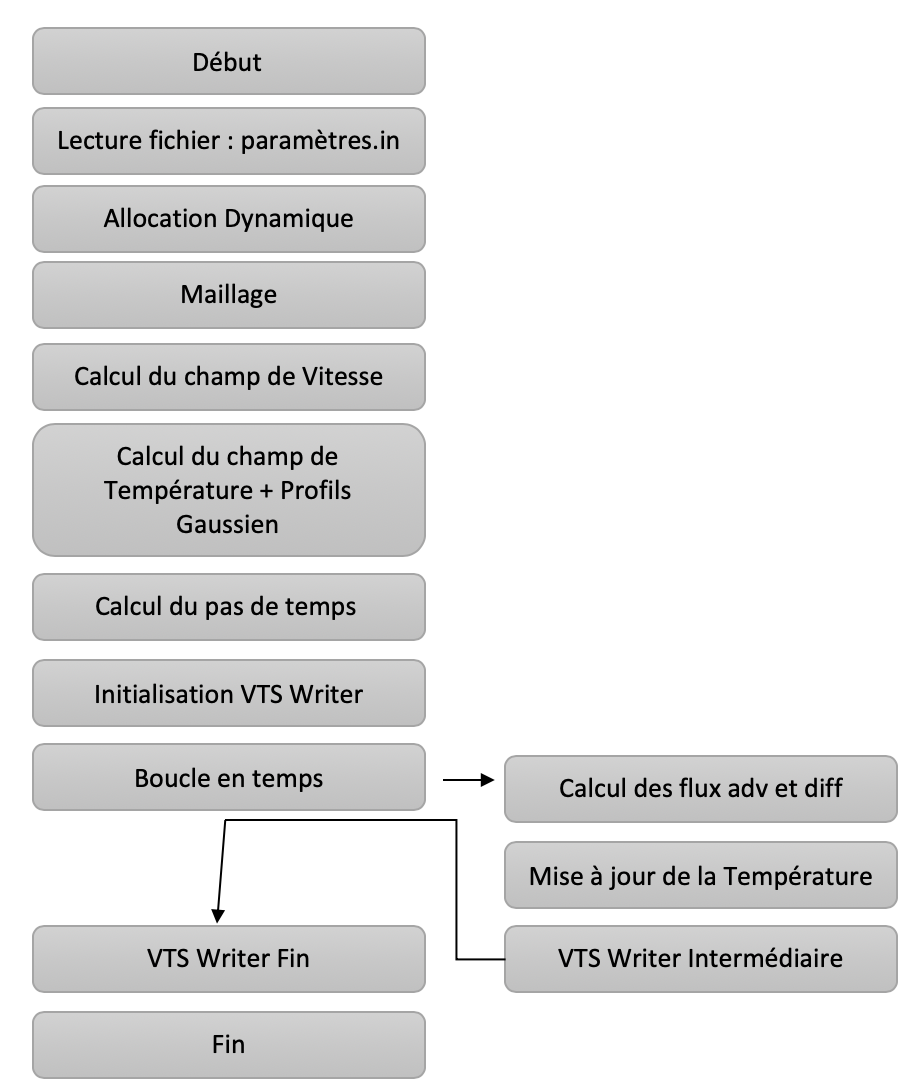
\includegraphics[scale=0.4]{Algo.PNG}
\caption{Algorigramme du calcul}
\end{figure}





\section{Validation}

\subsection{Construction du Champ des Vitesses}

Voici ce qu'on obtient en le modélisant sur ParaView, on observe bien la symétrie des deux profils de vitesse.

\begin{figure}[h!]
\centering
        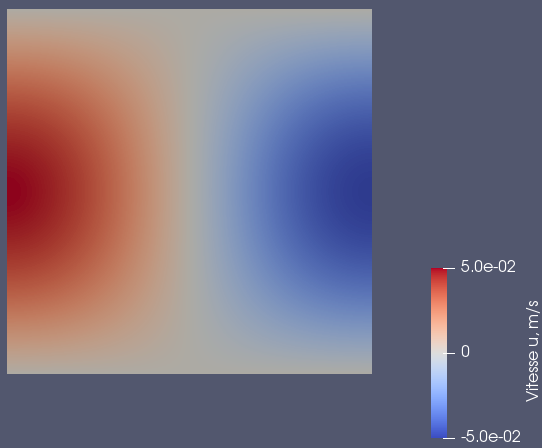
\includegraphics[scale=0.4]{Champ_Vitesse_Maillage/Champ_Vitesse_u.png}
        \caption{Champ des vitesses sur $u$ pour un maillage (100,100)}

\end{figure}

\begin{figure}[h!]
	\centering
        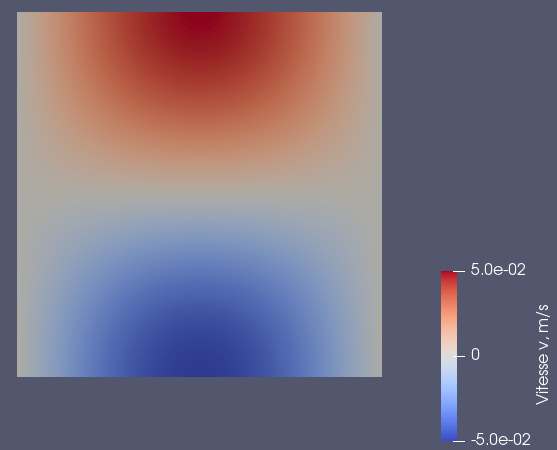
\includegraphics[scale=0.4]{Champ_Vitesse_Maillage/Champ_Vitesse_v.png}
        \caption{Champ des vitesses sur $v$ pour un maillage (100,100)}
\end{figure}


\subsection{Advection Pure 1D}

En fixant $u$ alternativement positive et négative et $v$ nulle et en prenant une température constante en entrée, on observe bien l'advection le phénomène d'advection pure.

\begin{figure}[h!]
\centering
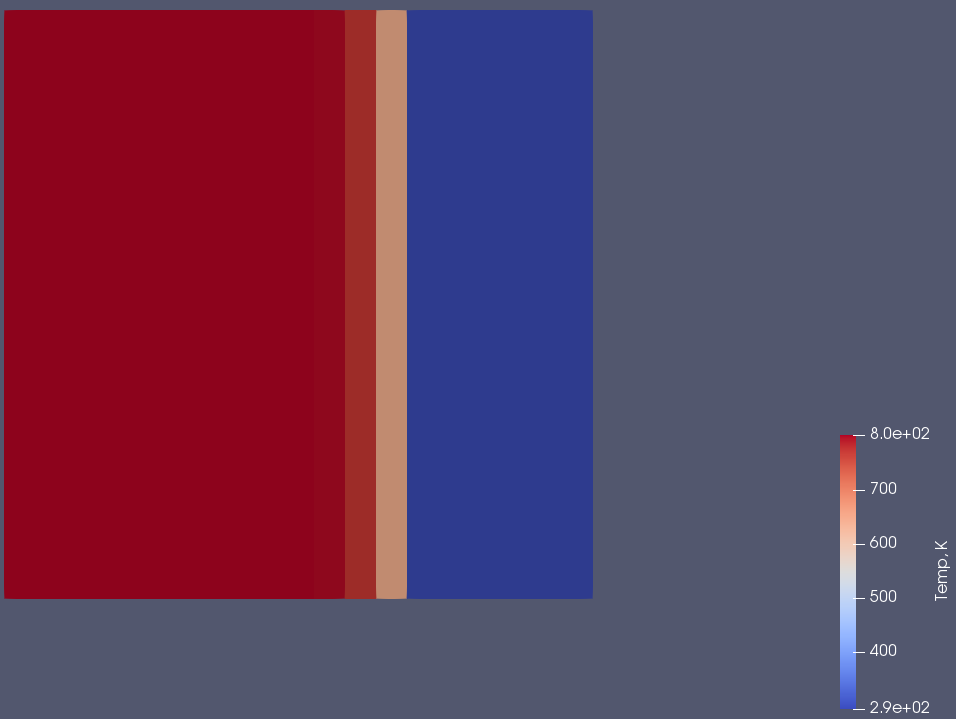
\includegraphics[scale=0.3]{Advection_Pure_1D/AdvGauche.png}
\caption{Température pour $u$ positive  (20,20), Ici on peut voir que le coefficient de diffusivité thermique n'est pas pris égal à 0}

\end{figure}

\begin{figure}[h!]
\centering
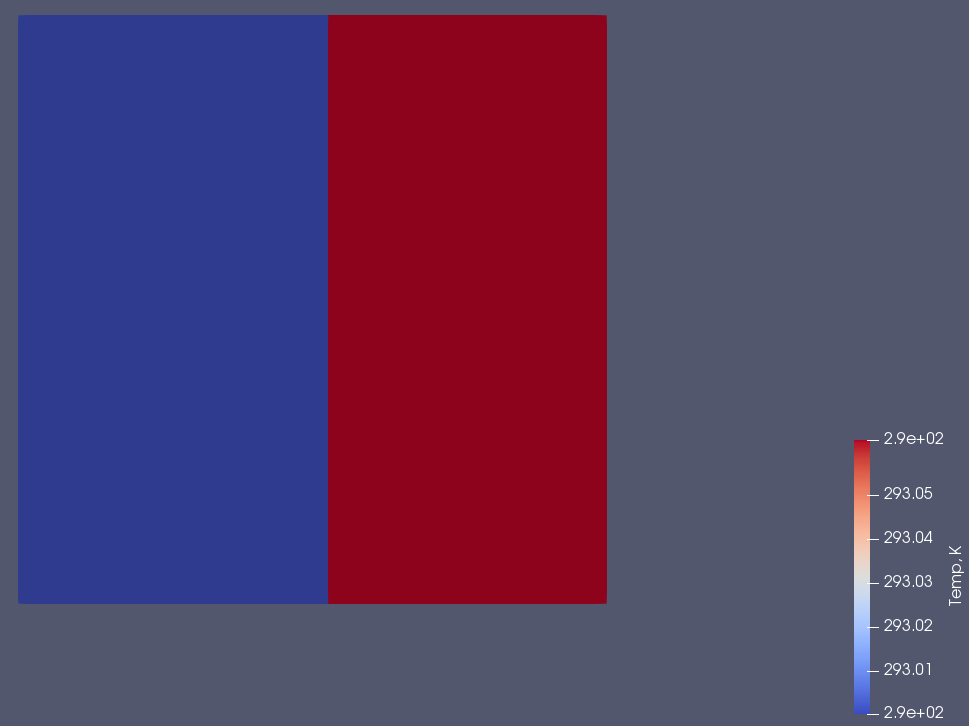
\includegraphics[scale=0.3]{Advection_Pure_1D/AdvDroite.png}
\caption{Température pour $u$ négative (51,51)}
\end{figure}


\subsection{Advection 2D}
En rétablissant alors le profil des vitesses avec la formule citée plus haut et en laissant une température constante en entrée on a alors :

\begin{figure}[h!]
\centering
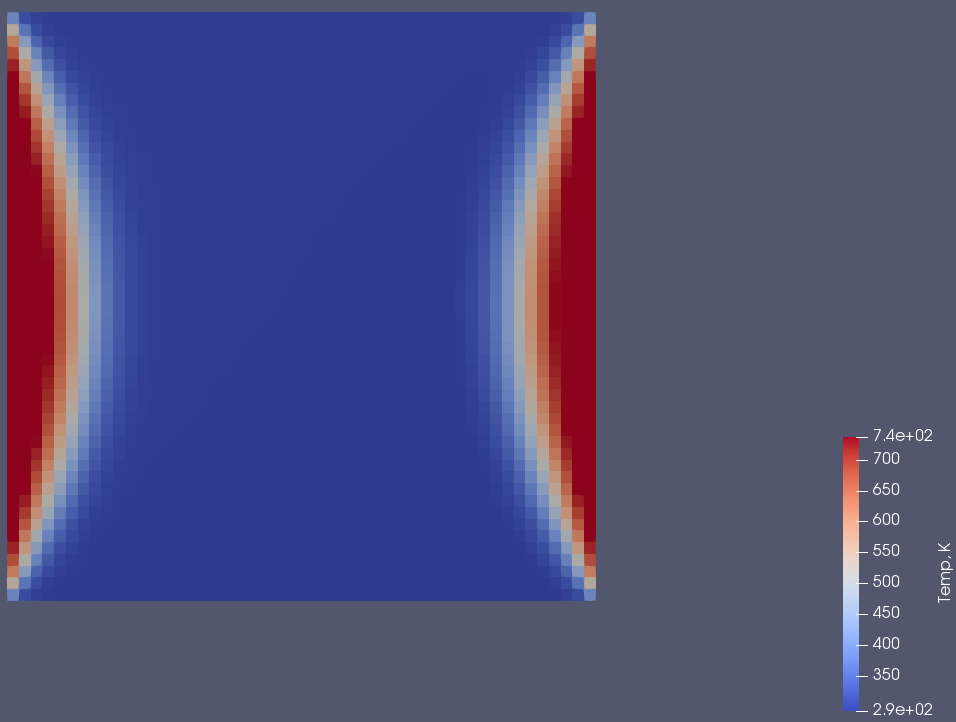
\includegraphics[scale=0.3]{Advection_2D/TemperatureStableEntree.png}
\caption{Température stable en entrée et $u$ et $v$ issues de \ref{eqvitesses} sur maillage (51,51)}
\end{figure}


\begin{figure}[h!]
\centering
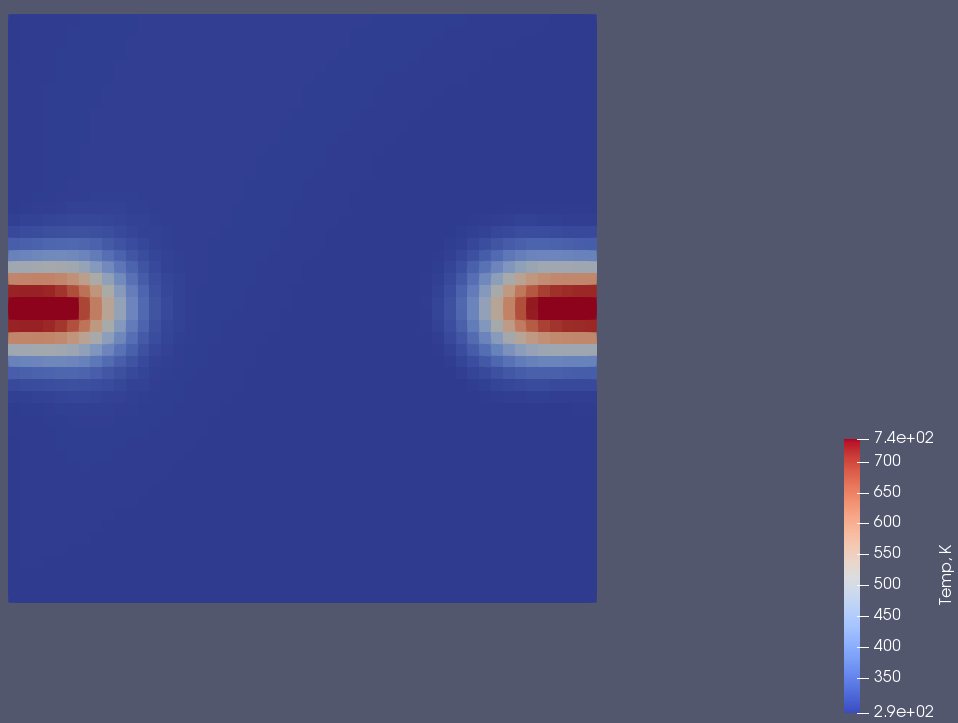
\includegraphics[scale=0.3]{Advection_2D/TemperatureGaussienne.png}
\caption{Température gaussienne en entrée et $u$ et $v$ issues de \ref{eqvitesses} sur maillage (51,51)}
\end{figure}



\section{Exploitation}


\section{Conclusion}



\end{document}
